\documentclass[11pt,compress,t,notes=noshow, aspectratio=169, xcolor=table]{beamer}

\usepackage{../../style/lmu-lecture}
% Defines macros and environments
% This file is included in slides and exercises

% Rarely used fontstyle for R packages, used only in 
% - forests/slides-forests-benchmark.tex
% - exercises/single-exercises/methods_l_1.Rnw
% - slides/cart/attic/slides_extra_trees.Rnw
\newcommand{\pkg}[1]{{\fontseries{b}\selectfont #1}}

% Spacing helpers, used often (mostly in exercises for \dlz)
\newcommand{\lz}{\vspace{0.5cm}} % vertical space (used often in slides)
\newcommand{\dlz}{\vspace{1cm}}  % double vertical space (used often in exercises, never in slides)
\newcommand{\oneliner}[1] % Oneliner for important statements, used e.g. in iml, algods
{\begin{block}{}\begin{center}\begin{Large}#1\end{Large}\end{center}\end{block}}

% Don't know if this is used or needed, remove?
% textcolor that works in mathmode
% https://tex.stackexchange.com/a/261480
% Used e.g. in forests/slides-forests-bagging.tex
% [...] \textcolor{blue}{\tfrac{1}{M}\sum^M_{m} [...]
% \makeatletter
% \renewcommand*{\@textcolor}[3]{%
%   \protect\leavevmode
%   \begingroup
%     \color#1{#2}#3%
%   \endgroup
% }
% \makeatother


\title{Interpretable Machine Learning}
% \author{LMU}
%\institute{\href{https://compstat-lmu.github.io/lecture_iml/}{compstat-lmu.github.io/lecture\_iml}}
\date{}

\bibliography{feature-importance}
%\usepackage{Sweave}

%\usepackage{Sweave}
\begin{document}
	\newcommand{\titlefigure}{figure_man/feature-importance.png}
    \newcommand{\learninggoals}{
    	\item Underdstand how PFI is computed
    	\item Understanding strengths and weaknesses
    	\item Testing Importance}
	% Set style/preamble.Rnw as parent.
	
	% Load all R packages and set up knitr
	
	% This file loads R packages, configures knitr options and sets preamble.Rnw as 
	% parent file
	% IF YOU MODIFY THIS, PLZ ALSO MODIFY setup.Rmd ACCORDINGLY...
	
	% Defines macros and environments

	\lecturechapter{Shapley Additive Global Importance (SAGE)}
	\lecture{Interpretable Machine Learning}
	
	% ------------------------------------------------------------------------------

% CHALLENGE
\begin{vbframe}{Challenge: Fair Attribution of Importance}
\textbf{Recap:} Data: $x_1, \dots, x_4$ uniformly sampled from $\{-1, 1\}$ and $y:= x_1 x_2 + x_3 + \epsilon_Y$ with $\epsilon_Y \sim N(0, 1)$. Model: $\fh(x) \approx x_1 x_2 + x_3$.\\

\begin{figure}
\centering
  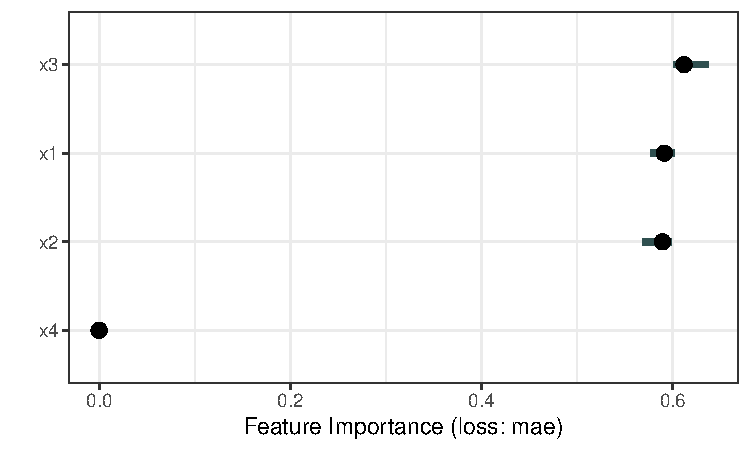
\includegraphics[width=0.5\linewidth]{figure_man/pfi_interactions.pdf}
\end{figure}

Although $x_3$ alone contributes as much to the performance as $x_1$ and $x_2$ jointly, all three are considered equally relevant by PFI.\\
\lz
Why? PFI assesses importance given that all remaining covariates are preserved. If we were to first permute $x_1$ and then $x_2$, the permutation of $x_2$ would have no effect on the performance (and vice versa).
\end{vbframe}


\begin{vbframe}{Challenge: Fair attribution of importance}

\textbf{Observation:} Feature importance attribution can be regarded as cooperative game, where each feature is a player and model performance is the payoff. The surplus contribution of a feature depends on the coalition of features that are already in the room.\\
\lz
\textbf{SAGE Idea:} Leverage game-theoretic Shapley values to compute a fair attribution of importance.\\
\lz
$\Rightarrow$ SAGE translates SHAP into a global feature importance technique\\
\lz
In order to compute SAGE, approximate Shapley values $\phi_j$ as for SHAP, replacing SHAP value functions with SAGE value functions.\\

\footnote[frame]{\fullcite{NEURIPS2020_c7bf0b7c}}
  
\end{vbframe}


% SAGE IDEA
\begin{vbframe}{SAGE Removal and Value function}
  
 \textbf{Removal Idea:} In order to deprive the model of the non-coalition features $-S$, marginalize the prediction function over the dropped features.

$$\fh_S(x_S) = \E[\fh(x) | X_S = x_S]$$
  
The dropped features can either be sampled from the marginal distribution $\P(x_{-S})$ or the conditional distribution $\P(x_{-S}|x_S)$.\\
\lz

\footnote[frame]{\fullcite{NEURIPS2020_c7bf0b7c}}

For SAGE, value functions quantify the predictive power of a coalition $S$ in terms of reduction in risk over the mean prediction.\\
\lz
Value function:  $ v_{\fh}(S) = \risk(\fh_{\emptyset}) - \risk(\fh_{S})$\\
\lz
Contribution of feature $x_j$ over coalition $x_S$:  $v_{\fh}(S \cup \{j\}) - v_{\fh}(S)$\\
\lz

\end{vbframe}

\begin{vbframe}[allowframebreaks]{SAGE Removal and Value function}

Depending on whether conditional or marginal resampling is used, the interpretation of SAGE value functions differ.\\
\lz
\textbf{Marginal resampling:} $v(S)$ quantifies the reliance of the model on features $x_S$
\begin{itemize}
  \item features $x_S$ not being causal for the prediction is a sufficient condition for $v(S) = 0$
\end{itemize}

\textbf{Conditional resampling}: $v(S)$ quantifies the reliance of the model on the information contained in variables $x_S$.
\begin{itemize}
  \item features $x_S$ not being causal for the prediction is not a sufficient condition for $v(S) = 0$
  \item under model optimality, links to mutual information or the conditional variance can be drawn
\end{itemize}

\framebreak

When the loss-optimal model $f^*$ is inspected using \textit{conditional-sampling} based SAGE value functions, interesting links exist.
\begin{itemize}
  \item \textbf{for cross-entropy loss:} the value function $v_{f^*}(S) = I(y;x_S)$ corresponds to the mutual information and the surplus contribution of a feature $x_j$ $v_{f^*}(S \cup \{j\}) - v_{f^*}(S) = I(y,x_i|x_S)$ to the conditional mutual information
  \item \textbf{for MSE loss:} the value function $v_{f^*}(S) = Var(y) - \E[Var(y|x_S)]$ corresponds to the expected reduction in variance given knowledge of the features $x_S$ and the surplus contribution $v_{f^*}(S \cup \{j\}) - v_{f^*}(S) = \E[Var(y|x_S)] - \E[Var(y|x_{S \cup {j}})]$ to the respective reduction over $x_S$
\end{itemize}

\framebreak

\textbf{Example:} $x_1 = \epsilon_1$, $x_2 = x_1 + \epsilon_2$, $x_3 = x_2 + \epsilon_3$, $y = x_3 + \epsilon_y$ with $\epsilon_j$ independent noise terms (causal DAG: $x_1 \rightarrow x_2 \rightarrow x_3 \rightarrow y$). The prediction model is defined as  $\fh \approx 0.95 x_3 + 0.05 x_2$. 
%
\begin{figure}
  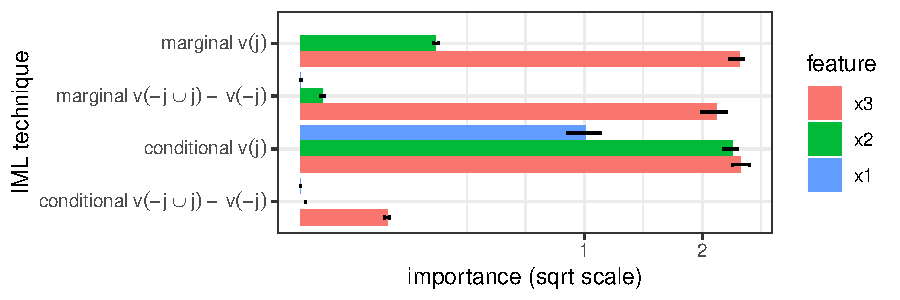
\includegraphics[width=0.6\linewidth]{figure_man/sage_variants}
\end{figure}
%
While the conditional $v(j)$ are nonzero for features that are not used by $\fh$, marginal $v(j)$ are only nonzero for features that are used by $\fh$. 
Since for conditional $v$ the difference $v(-j \cup j) - v(-j)$ quantifies the unique contribution of $x_j$ over remaining variables $-j$ and $y \indep x_1, x_2 | x_3$, only $v(\{1,2,3\}) - v(\{1, 2\})$ is nonzero.
%
\end{vbframe}

\begin{vbframe}{SAGE interpretation}

The Shapley axioms can be translated into properties of SAGE. The interpretation depends on whether conditional or marginal sampling is used.
%
\begin{table}
  \centering
  \begin{tabular}{l | l }
  Shapley property $\implies$ & conditional SAGE property \\
  \hline
  efficiency & $\sum_{i=1}^d \phi_j(v) = \risk(\fh_\emptyset) - \risk(\fh)$\\
  symmetry & $x_j = x_i \implies \phi_i = \phi_j$ \\
  linearity & $\phi_j$ expecation of per-instance\\
  & conditional SHAP applied to model loss\\
  monotonicity & given models $f, f'$, if  $\forall S:$\\
  &$v_f(S \cup j) - v_f(S) \geq v_{f'}(S \cup j) - v_{f'}(S)$ \\
  &then $\phi_j(v_f) \geq \phi_j(v_{f'})$\\
  dummy & if $\forall S: \fh(x) \indep x_j | x_S \Rightarrow \phi_j = 0$
  \end{tabular}
\end{table}

\end{vbframe}

\begin{vbframe}{SAGE interpretation}
%
The Shapley axioms can be translated into properties of SAGE. The interpretation depends on whether conditional or marginal sampling is used.
%
\begin{table}
  \centering
  \begin{tabular}{l | l }
  Shapley property $\implies$ & marginal SAGE property \\
  \hline
  efficiency & $\sum_{i=1}^d \phi_j(v) = \risk(\fh_\emptyset) - \risk(\fh)$\\
  symmetry & no intelligible implication \\
  linearity & $\phi_j$ expecation of per-instance\\
  & marginal SHAP applied to model loss\\
  monotonicity & given models $f, f'$, if  $\forall S:$\\
  &$v_f(S \cup j) - v_f(S) \geq v_{f'}(S \cup j) - v_{f'}(S)$ \\
  &then $\phi_j(v_f) \geq \phi_j(v_{f'})$\\
  dummy & model invariant to $x_j \Rightarrow \phi_j = 0$\\
  \end{tabular}
\end{table}
%
\end{vbframe}

\begin{vbframe}{Interaction Example Revisited}

\textbf{Recap:} Data: $x_1, \dots, x_4$ uniformly sampled from $\{-1, 1\}$ and $y:= x_1 x_2 + x_3 + \epsilon_Y$ with $\epsilon_Y \sim N(0, 1)$. Model: $\fh(x) \approx x_1 x_2 + x_3$.\\
%
\begin{figure}
  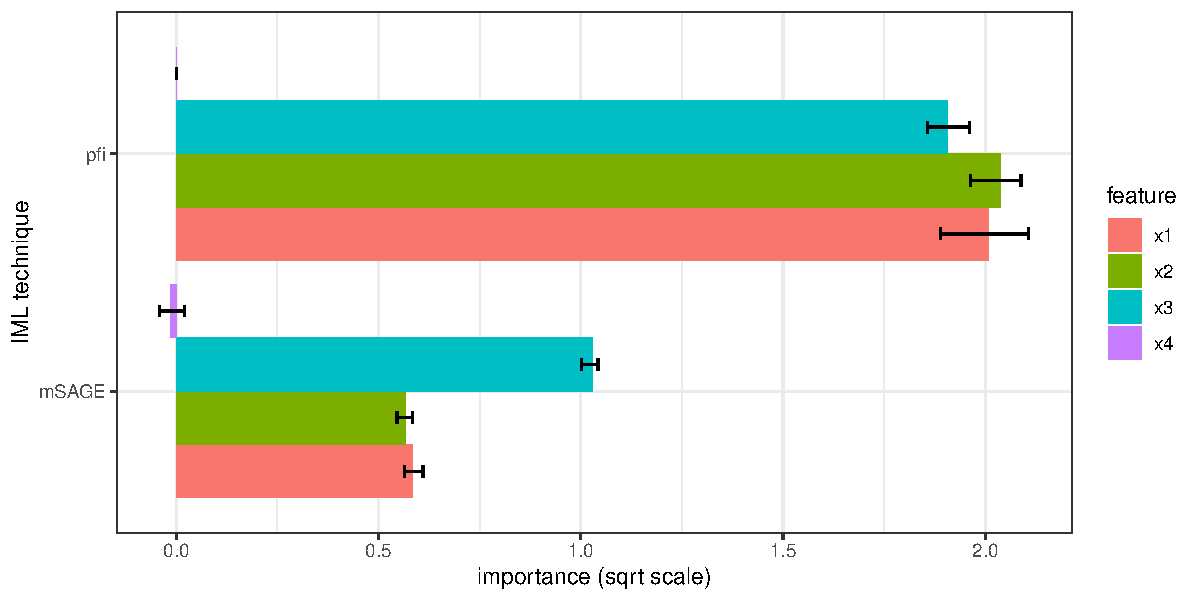
\includegraphics[width=0.7\linewidth]{figure_man/sage_pfi_interactions}
\end{figure}
%
While PFI regards $x_1, x_2$ to be equally important as $x_3$, marginal SAGE fairly divides the contribution of the interaction $x_1$ and $x_2$.
  
\end{vbframe}


%\begin{vbframe}{Implications marginal SAGE}
%
%Can we gain insight into whether...
%
%\begin{enumerate}
%    \item the feature $x_j$ is causal for the prediction?
%    \begin{itemize}
%      \item yes, because of the dummy property nonzero $\phi_j$ implies $x_j \rightarrow \fh(x)$
%    \end{itemize}
%    \item the variable $x_j$ contains prediction-relevant information?
%    \begin{itemize}
%      \item No, whether a model relies on the feature (to improve the performance).
%    \end{itemize}
%    \item the model requires access to $x_j$ to achieve it's prediction performance?    
%    \begin{itemize}
%      \item 
%\end{itemize}
%\end{enumerate}
%
%\end{vbframe}
%
%\begin{vbframe}{Implications conditional SAGE}
%
%Can we gain insight into whether...
%
%\begin{itemize}
%    \item the feature $\xj$ is causal for the prediction?
%    \begin{itemize}
%      \item no
%    \end{itemize}
%    \item the variable $\xj$ contains prediction-relevant information about $\ydat$?
%    \begin{itemize}
%      \item yes
%    \end{itemize}
%    \item the model requires access to $x_j$ to achieve it's prediction performance?  
%    \begin{itemize}
%        \item no
%    \end{itemize}
%\end{itemize}
%
%\end{vbframe}


\begin{vbframe}
  \printbibliography
\end{vbframe}

\endlecture
\end{document}
